\documentclass[conference]{IEEEtran}

\usepackage{amsmath}
\usepackage{booktabs}
\usepackage{cite}
\usepackage{graphicx}
\usepackage{xurl}

\graphicspath{{../charts/}}

\title{Stablecoin Peg Stability and Risk-Aware Capital Allocation in DeFi}

\author{
\IEEEauthorblockN{Engin Samet Dede}
\IEEEauthorblockA{
University of Geneva\\
Geneva, Switzerland\\
GitHub: \url{https://github.com/Engn21}
}
}

\begin{document}

\maketitle

\begin{abstract}
Stablecoins are widely treated as interchangeable dollar-denominated assets in decentralized finance (DeFi), yet their peg behavior is shaped by different collateral, governance, liquidity, and redemption mechanisms. This paper studies the peg stability of four major stablecoins--USDT, USDC, DAI, and FRAX--using daily USD price and trading-volume data collected from the CoinGecko public API over a rolling 365-day window. The analysis measures absolute peg deviation, de-peg frequency, rolling volatility, volume-weighted deviation, and correlation with broad crypto-market stress. The results show that stablecoin risk is not homogeneous: fiat-collateralized stablecoins maintain the tightest day-to-day peg but concentrate counterparty and custody risk; DAI exhibits a more observable on-chain risk profile; and FRAX shows wider deviation behavior linked to its hybrid design. A Kruskal-Wallis test reported by the accompanying notebook indicates statistically distinct deviation distributions across the four assets. The findings support portfolio policies that disaggregate stablecoin exposure by mechanism and continuously monitor peg deviation rather than treating all stablecoins as generic one-dollar instruments.
\end{abstract}

\begin{IEEEkeywords}
Stablecoins, DeFi, peg stability, market risk, capital allocation, non-parametric testing.
\end{IEEEkeywords}

\section{Introduction}
Stablecoins are a core settlement and collateral instrument in DeFi. They are used in lending markets, automated market makers, derivatives collateral, treasury management, and yield strategies~\cite{schar_2021_defi}. Their apparent simplicity--a target value of one U.S. dollar--often hides meaningful differences in mechanism design and failure modes. A portfolio that treats USDT, USDC, DAI, and FRAX as equivalent cash-like assets may therefore underprice both continuous peg noise and discontinuous tail risk.

This research addresses the following question: how tightly do major stablecoins maintain their \$1 peg, under what conditions do they deviate, and what does this imply for risk-aware capital allocation in DeFi? The contribution is an empirical workflow that compares multiple stablecoin mechanisms using consistent deviation metrics and visual diagnostics. The analysis emphasizes both average behavior and stress behavior, because capital allocation is affected not only by normal-day tracking error but also by liquidity, recovery time, and market-correlation properties during shocks.

\section{Related Work}
Stablecoin research typically separates assets by the economic structure that supports the peg. Bullmann, Klemm, and Pinna propose a taxonomy based on issuer accountability, decentralization of responsibilities, and the asset backing the claim~\cite{bullmann_2019_stablecoins}. Klages-Mundt et al. formalize stablecoin risks across custodial and non-custodial designs~\cite{klages_2020_stablecoins2}. Lyons and Viswanath-Natraj show that stablecoin price stability is closely related to arbitrage, liquidity, and demand-side forces rather than issuance alone~\cite{lyons_2023_stablecoins}. Kozhan and Viswanath-Natraj study DAI specifically and link decentralized stablecoin peg deviations to collateral, arbitrage frictions, and CDP-level behavior~\cite{kozhan_2021_dai}.

The regulatory literature emphasizes redemption rights, reserve quality, run risk, and financial-stability spillovers. Gorton and Zhang compare stablecoins with private bank money and argue that issuer liabilities can be run-prone when par convertibility is uncertain~\cite{gorton_zhang_2023_wildcat}. The Financial Stability Board, BIS, IMF, and the U.S. President's Working Group all identify stablecoin-specific vulnerabilities around reserve assets, redemption, operational risk, and cross-border supervision~\cite{fsb_2023_gsc,bis_2022_future_monetary,imf_2021_gfsr,pwg_2021_stablecoins}. This paper connects that literature to a reproducible empirical workflow for measuring peg behavior across multiple stablecoin mechanisms.

\section{Assets and Mechanisms}
The study covers four stablecoins selected to represent distinct collateralization mechanisms. Table~\ref{tab:assets} summarizes the sample.

\begin{table}[t]
\caption{Stablecoins Included in the Study}
\label{tab:assets}
\centering
\begin{tabular}{lll}
\toprule
Asset & Ticker & Mechanism \\
\midrule
Tether & USDT & Fiat-collateralized, centralized \\
USD Coin & USDC & Fiat-collateralized, centralized \\
Dai & DAI & Crypto-collateralized, MakerDAO \\
Frax & FRAX & Fractional-algorithmic, hybrid \\
\bottomrule
\end{tabular}
\end{table}

The comparison is intentionally mechanism-aware. Fiat-collateralized stablecoins can exhibit low observed price variance while still carrying concentrated issuer, custodian, regulatory, and redemption risks~\cite{arner_auer_frost_2020_stablecoins,pwg_2021_stablecoins}. Crypto-collateralized designs such as DAI expose collateral and liquidation dynamics more transparently on-chain, but their peg can be affected by crypto-asset volatility and governance parameters~\cite{kozhan_2021_dai}. Fractional or hybrid designs add reflexive risk because endogenous collateral or governance-token value may deteriorate during the same stress periods in which redemptions increase~\cite{adams_ibert_2022_runs}.

\section{Data and Methodology}
Daily close prices and trading volumes are collected from the CoinGecko \texttt{/coins/\{id\}/market\_chart} endpoint~\cite{coingecko_api}. The notebook fetches data for the last 365 days at execution time, so the exact sample period changes when the analysis is rerun. Prices are denominated in U.S. dollars and cleaned by sorting, de-duplicating dates, trimming to the latest 365 observations, and forward-filling isolated missing values.

For stablecoin $i$ on date $t$, the absolute peg deviation is defined as
\begin{equation}
d_{i,t} = |p_{i,t} - 1|,
\end{equation}
where $p_{i,t}$ is the observed USD price. Two operational thresholds are used: a tight-peg band at $\pm0.5\%$ and a de-peg band at $\pm1.0\%$. A de-peg event is any day for which $d_{i,t}>0.01$, with direction classified as a premium when $p_{i,t}>1$ and a discount when $p_{i,t}<1$.

The study computes the following risk metrics for each asset:
\begin{itemize}
\item mean, median, and maximum absolute deviation;
\item standard deviation of daily absolute deviation;
\item number of days outside the $\pm0.5\%$ and $\pm1.0\%$ bands;
\item event recovery time, measured as consecutive days outside the $\pm1.0\%$ band;
\item 30-day rolling volatility of absolute deviation;
\item 30-day volume-weighted peg deviation;
\item Pearson correlation between absolute BTC daily returns and stablecoin deviation.
\end{itemize}

The volume-weighted deviation for stablecoin $i$ over rolling window $W_t$ is
\begin{equation}
\mathrm{VWDev}_{i,t} =
\frac{\sum_{\tau \in W_t} d_{i,\tau} v_{i,\tau}}
{\sum_{\tau \in W_t} v_{i,\tau}},
\end{equation}
where $v_{i,\tau}$ is reported trading volume. This prevents low-liquidity deviations from being interpreted the same way as high-volume deviations.

Finally, a Kruskal-Wallis test is used to evaluate whether the four deviation distributions are statistically identical. Pairwise Mann-Whitney U tests are then applied as post-hoc comparisons. These non-parametric tests are appropriate because peg-deviation distributions are heavy-tailed and not expected to be Gaussian.

\section{Empirical Results}
Fig.~\ref{fig:prices} shows daily prices relative to the \$1 peg with the $\pm0.5\%$ and $\pm1.0\%$ bands. The visual result is consistent with the main thesis: most observations are close to \$1, but the assets do not share the same dispersion and stress behavior.

\begin{figure*}[t]
\centering
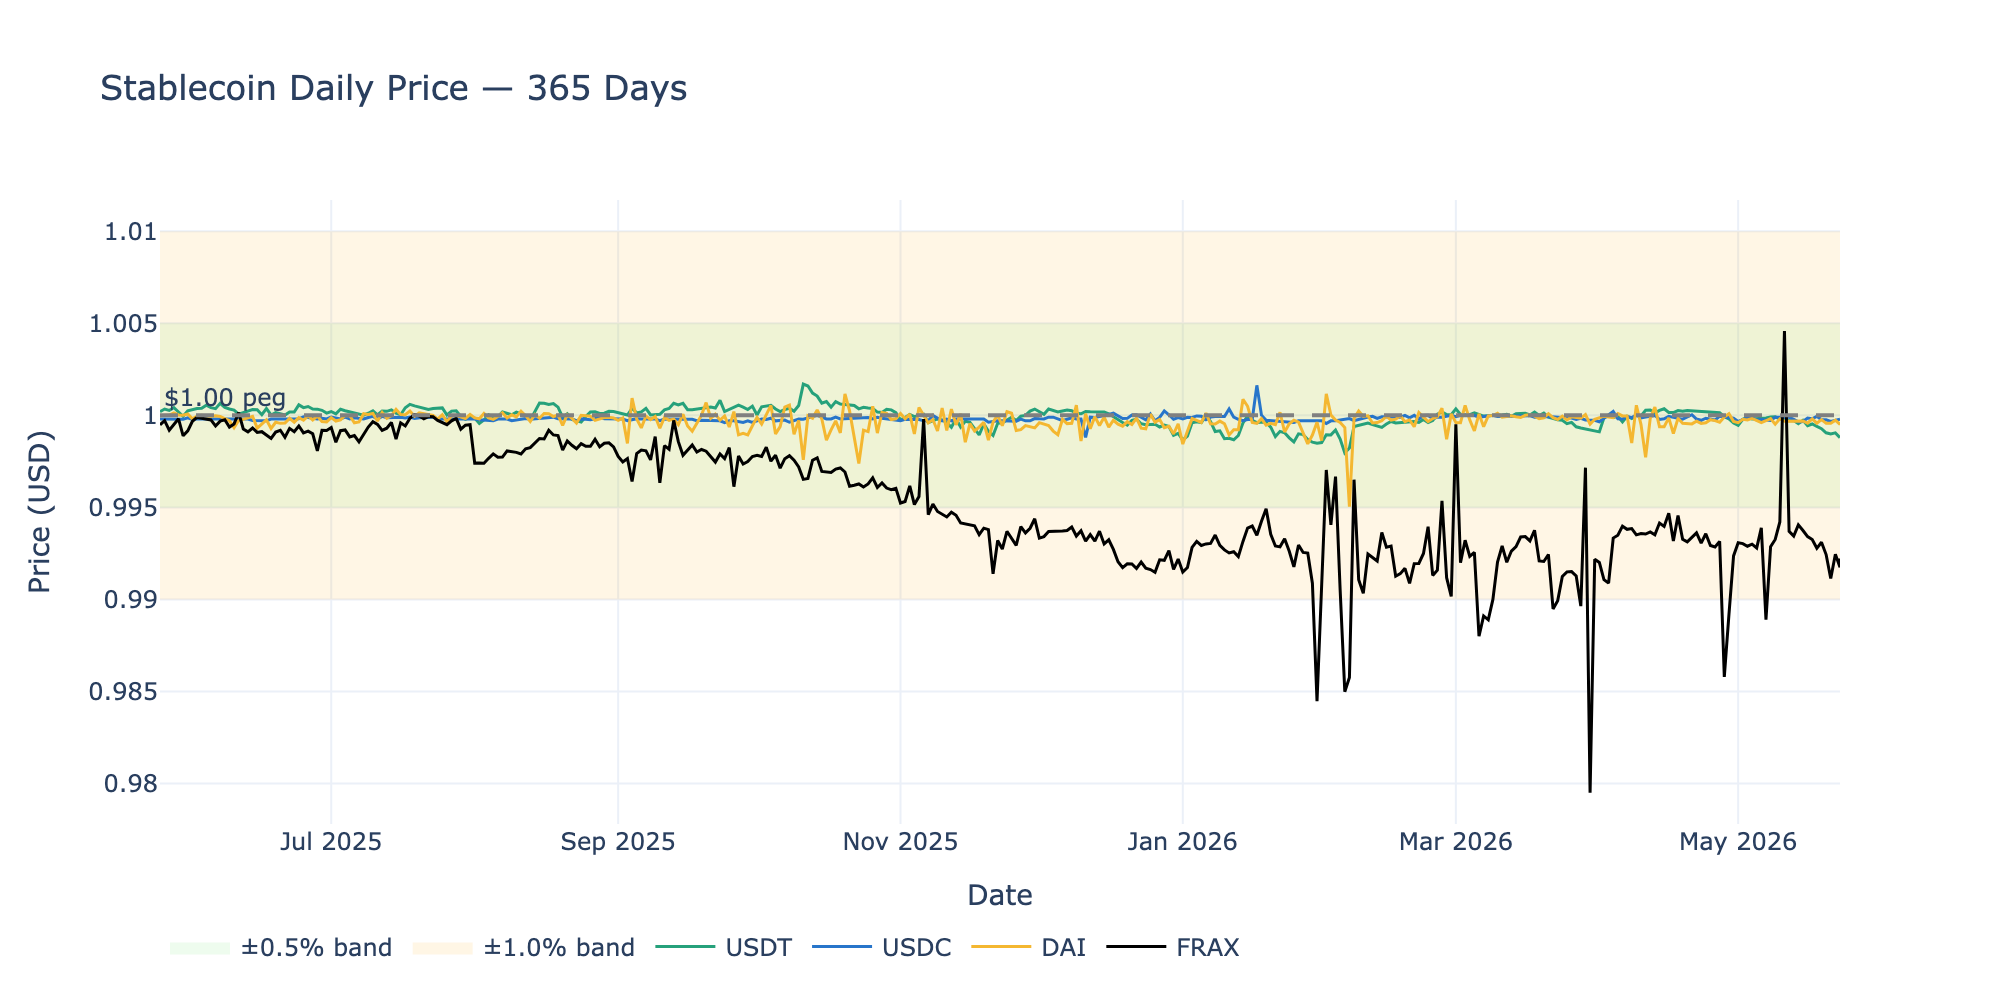
\includegraphics[width=0.92\textwidth]{price_timeseries.png}
\caption{Daily stablecoin prices around the \$1 peg. The shaded bands represent $\pm0.5\%$ and $\pm1.0\%$ thresholds.}
\label{fig:prices}
\end{figure*}

Fig.~\ref{fig:boxplot} compares the deviation distributions. The fiat-collateralized assets show the tightest day-to-day peg behavior, while DAI and FRAX show wider distributions. The accompanying notebook reports that the Kruskal-Wallis test rejects equality of the four distributions at the 5\% level, supporting separate treatment of each stablecoin in portfolio risk models.

\begin{figure}[t]
\centering
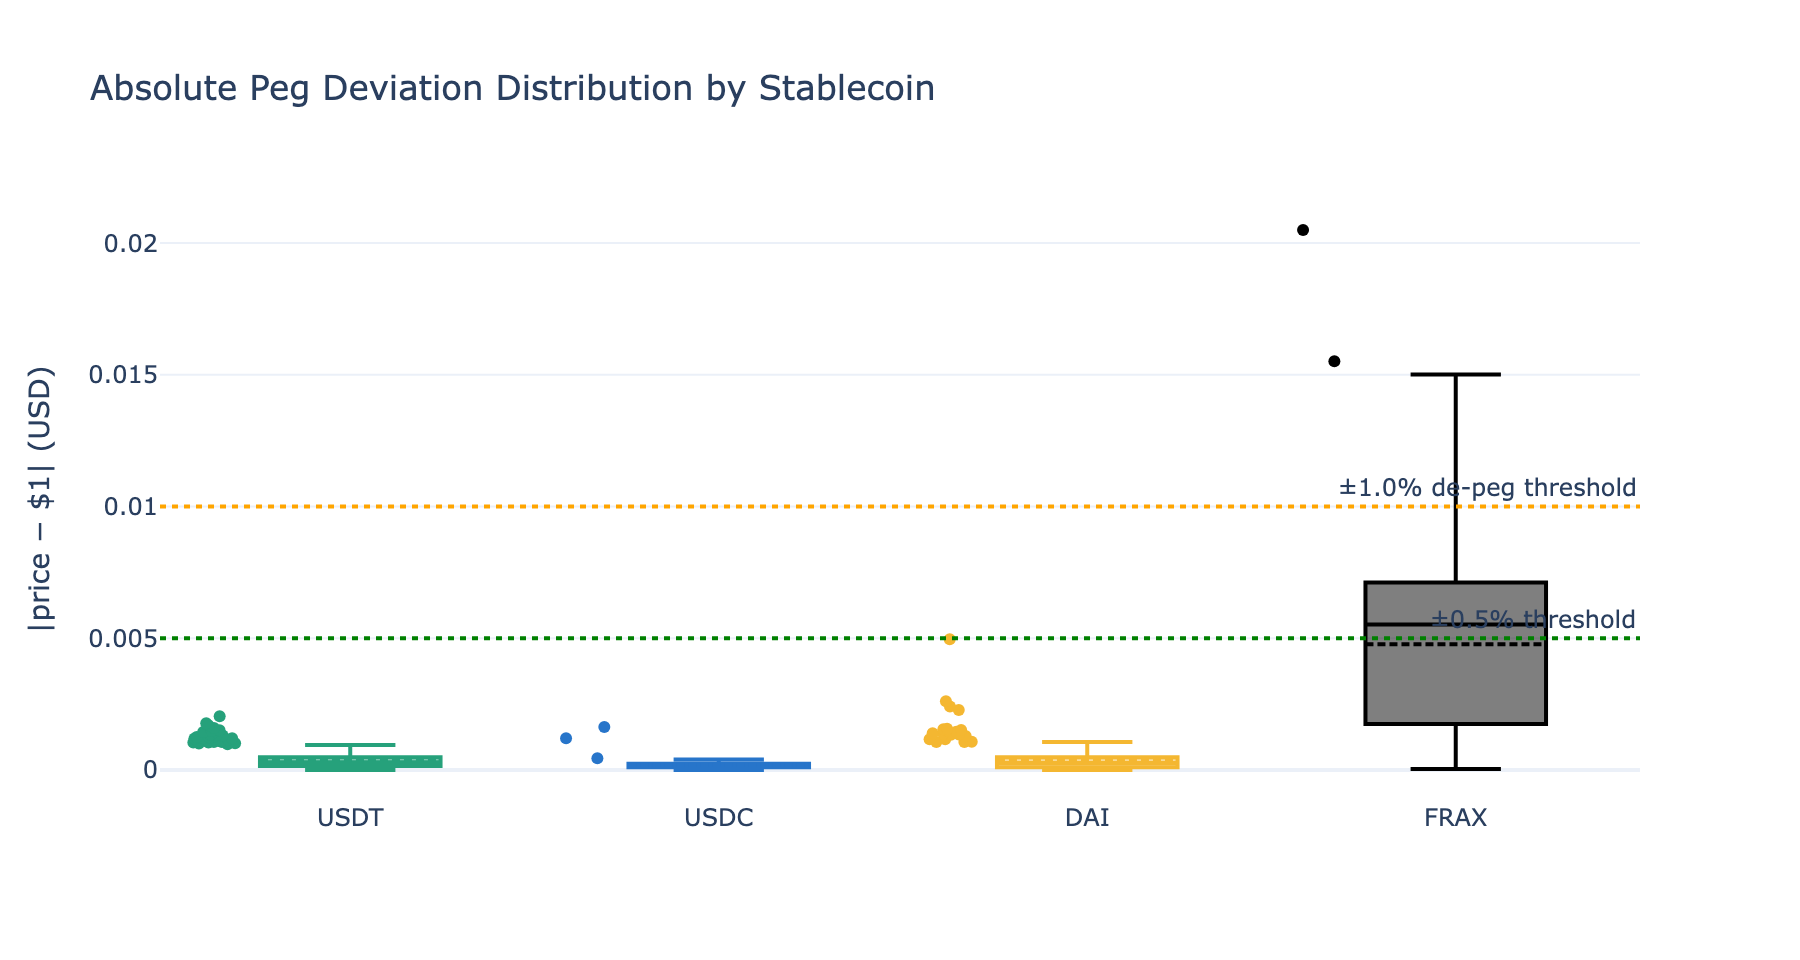
\includegraphics[width=\columnwidth]{deviation_boxplot.png}
\caption{Distribution of absolute peg deviation by stablecoin.}
\label{fig:boxplot}
\end{figure}

Monthly average deviations in Fig.~\ref{fig:heatmap} show that peg risk clusters through time. This matters for allocation because a fixed risk budget based only on full-sample averages can become stale when market conditions change.

\begin{figure}[t]
\centering
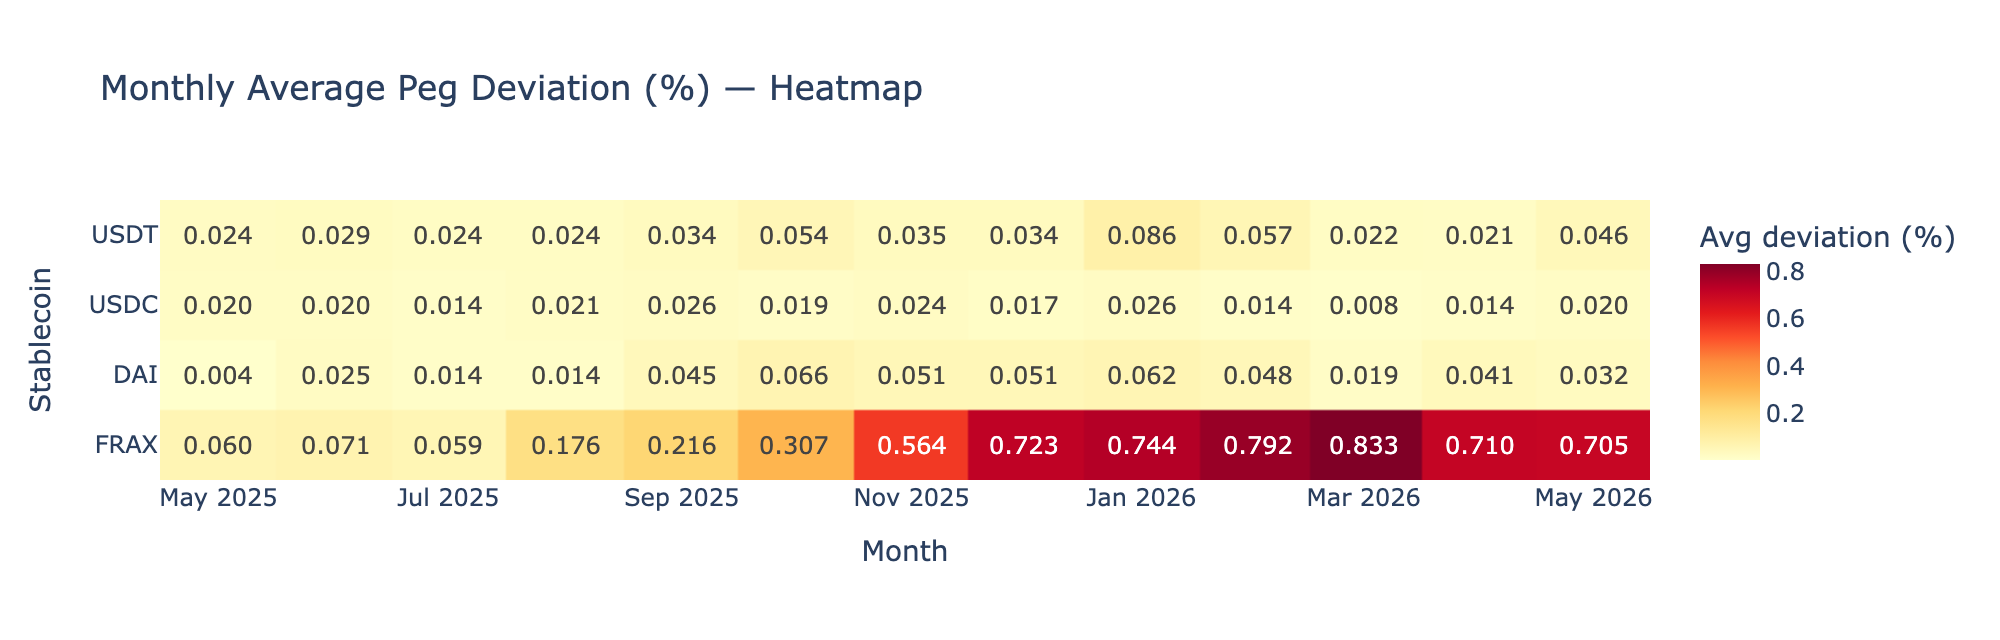
\includegraphics[width=\columnwidth]{monthly_heatmap.png}
\caption{Monthly average peg deviation. Darker cells indicate larger average deviation.}
\label{fig:heatmap}
\end{figure}

Fig.~\ref{fig:radar} aggregates normalized risk dimensions into a relative profile. The radar chart is not a substitute for a formal risk model, but it is useful for quickly comparing how each asset ranks across deviation magnitude, volatility, and threshold breaches.

\begin{figure}[t]
\centering
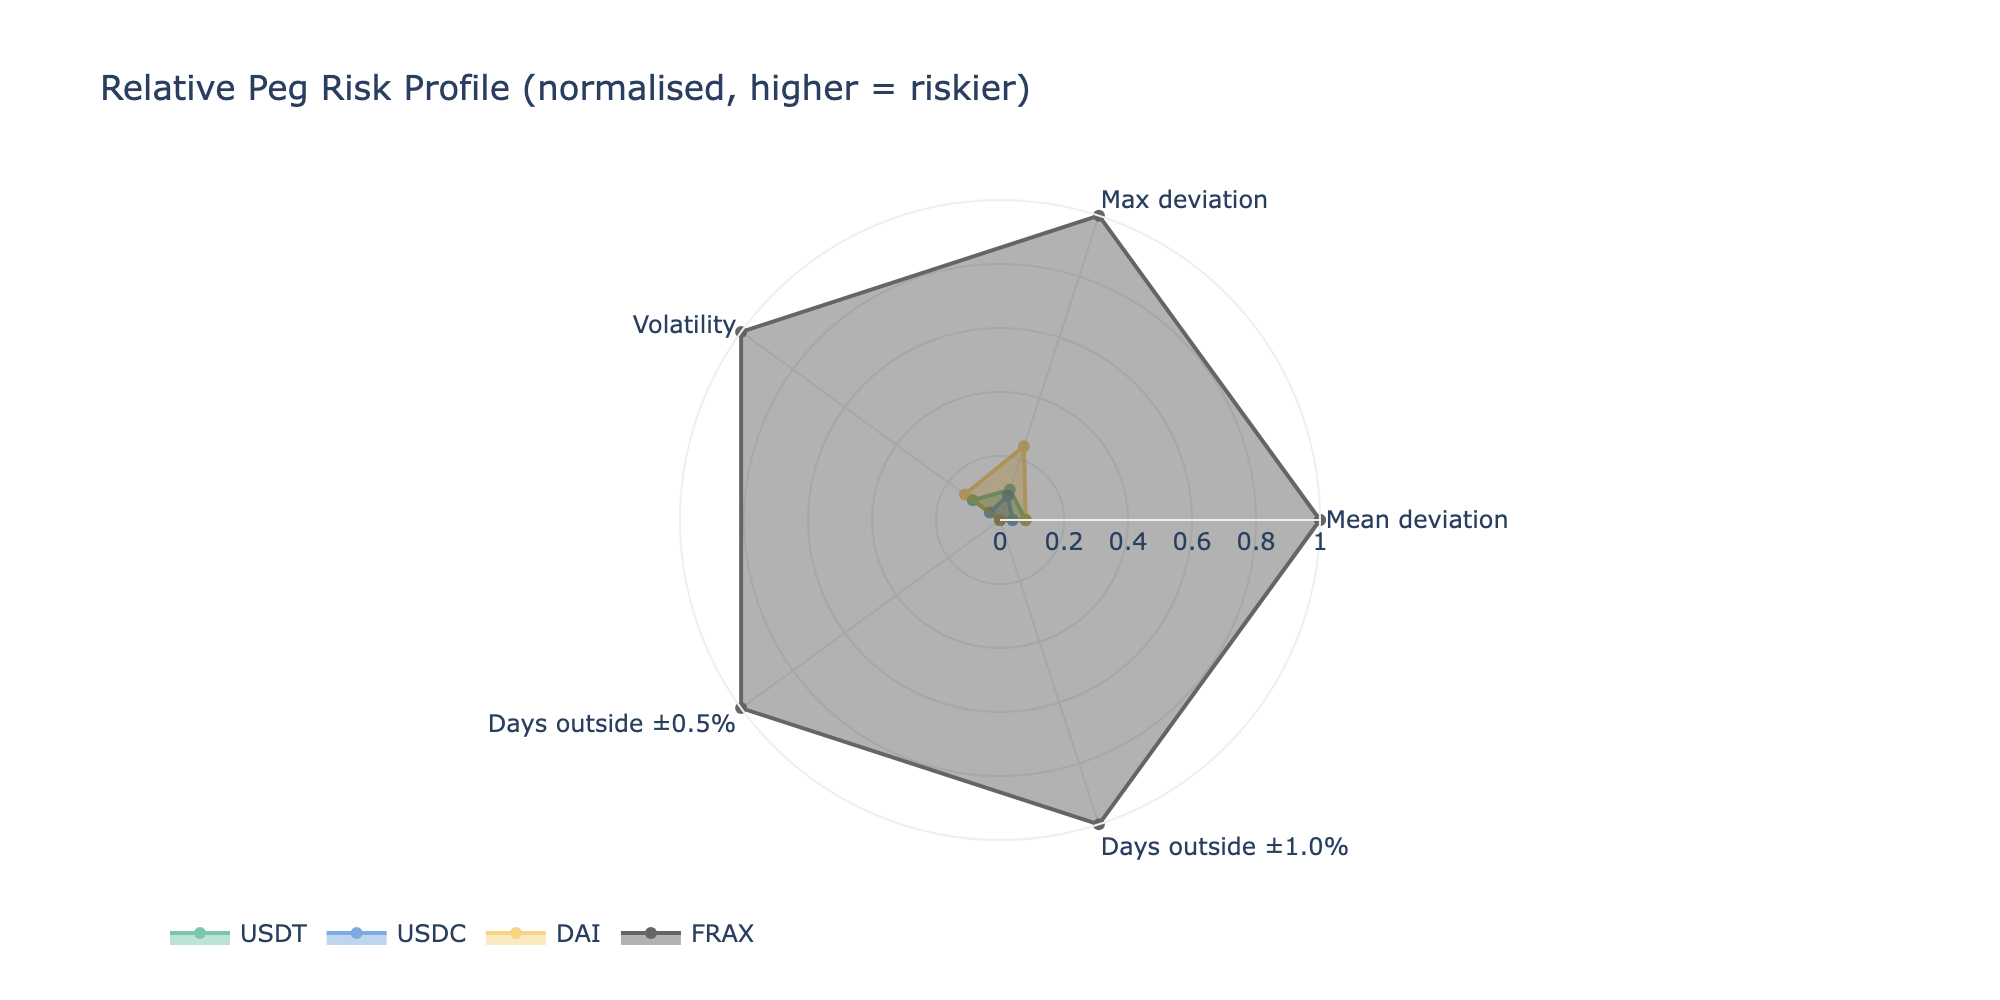
\includegraphics[width=\columnwidth]{risk_radar.png}
\caption{Normalized relative risk profile. Higher values indicate higher relative risk on the selected metric.}
\label{fig:radar}
\end{figure}

\section{Time-Varying and Liquidity-Adjusted Risk}
Static summary statistics can hide changes in risk regime. Fig.~\ref{fig:rolling} plots the 30-day rolling volatility of peg deviation. Periods of elevated rolling volatility indicate that peg risk is time-varying and should be monitored dynamically rather than assumed constant.

\begin{figure}[t]
\centering
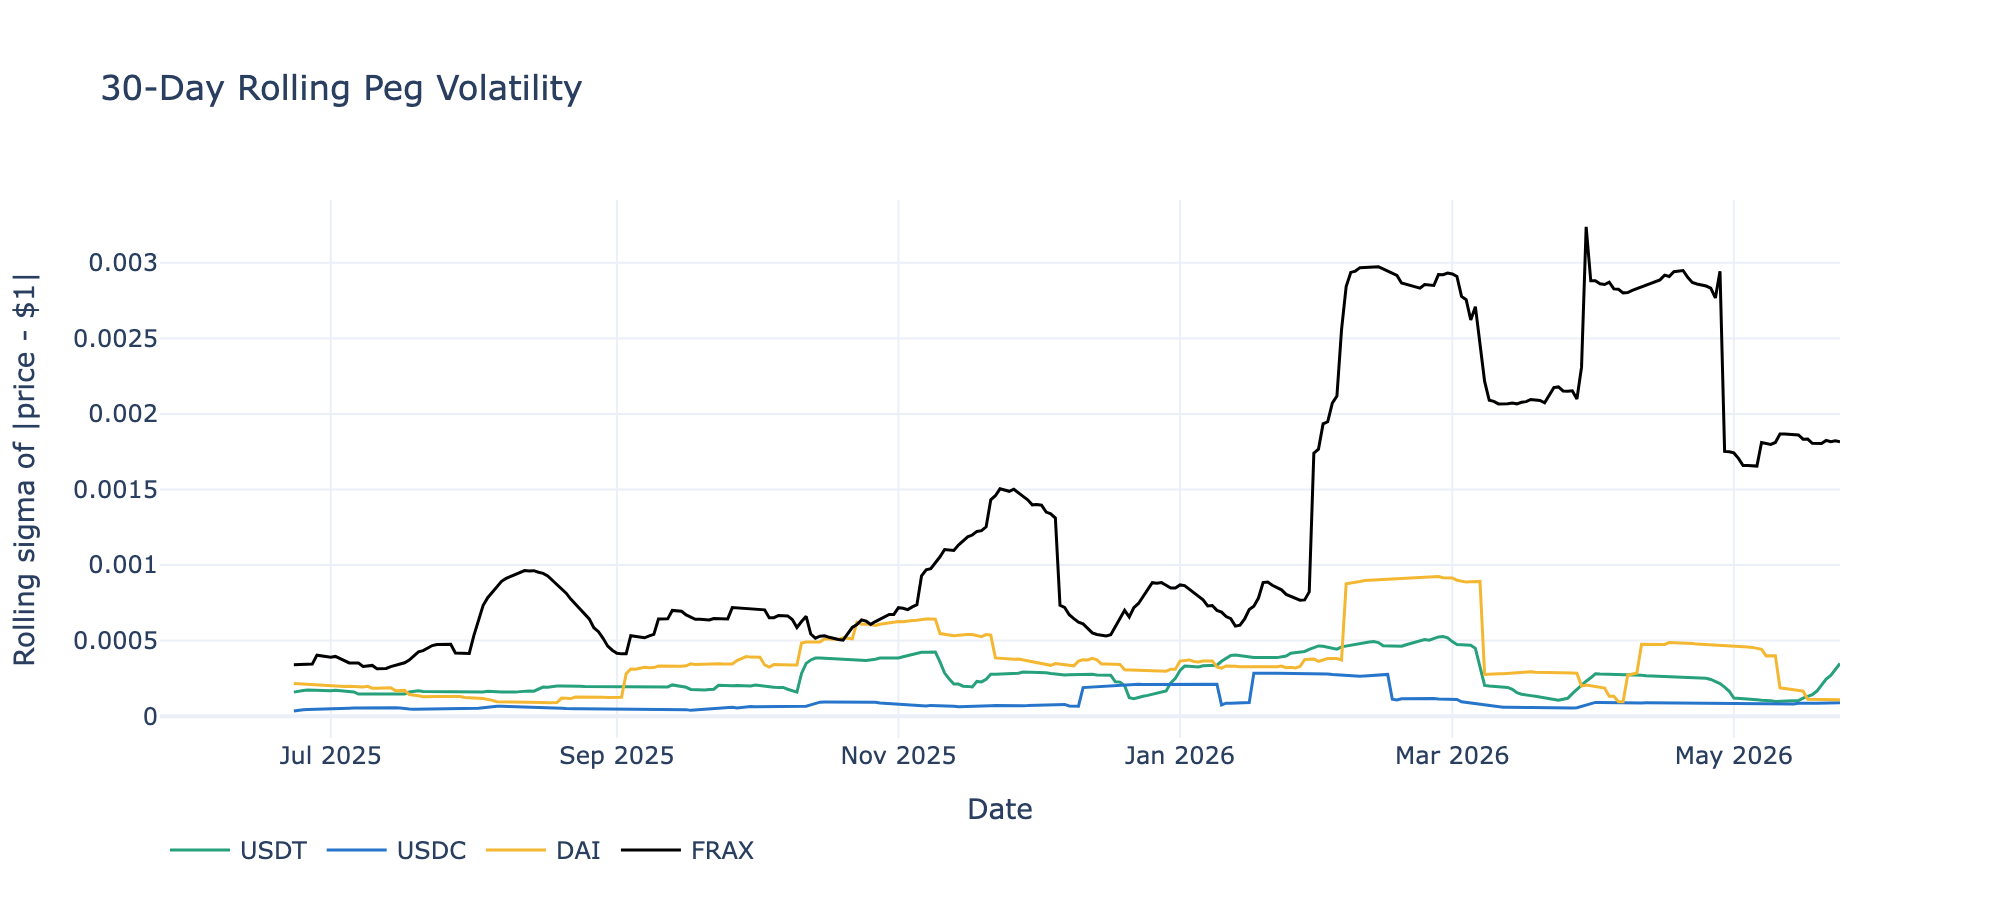
\includegraphics[width=\columnwidth]{rolling_volatility.png}
\caption{Thirty-day rolling volatility of absolute peg deviation.}
\label{fig:rolling}
\end{figure}

Fig.~\ref{fig:vwdev} reports 30-day volume-weighted deviation. This liquidity-adjusted measure is important for capital deployment because a deviation on thin volume has different implications from a deviation during heavy trading activity. Volume-weighting therefore helps identify deviations that are more likely to matter for large positions, liquidations, and redemption pressure.

\begin{figure}[t]
\centering
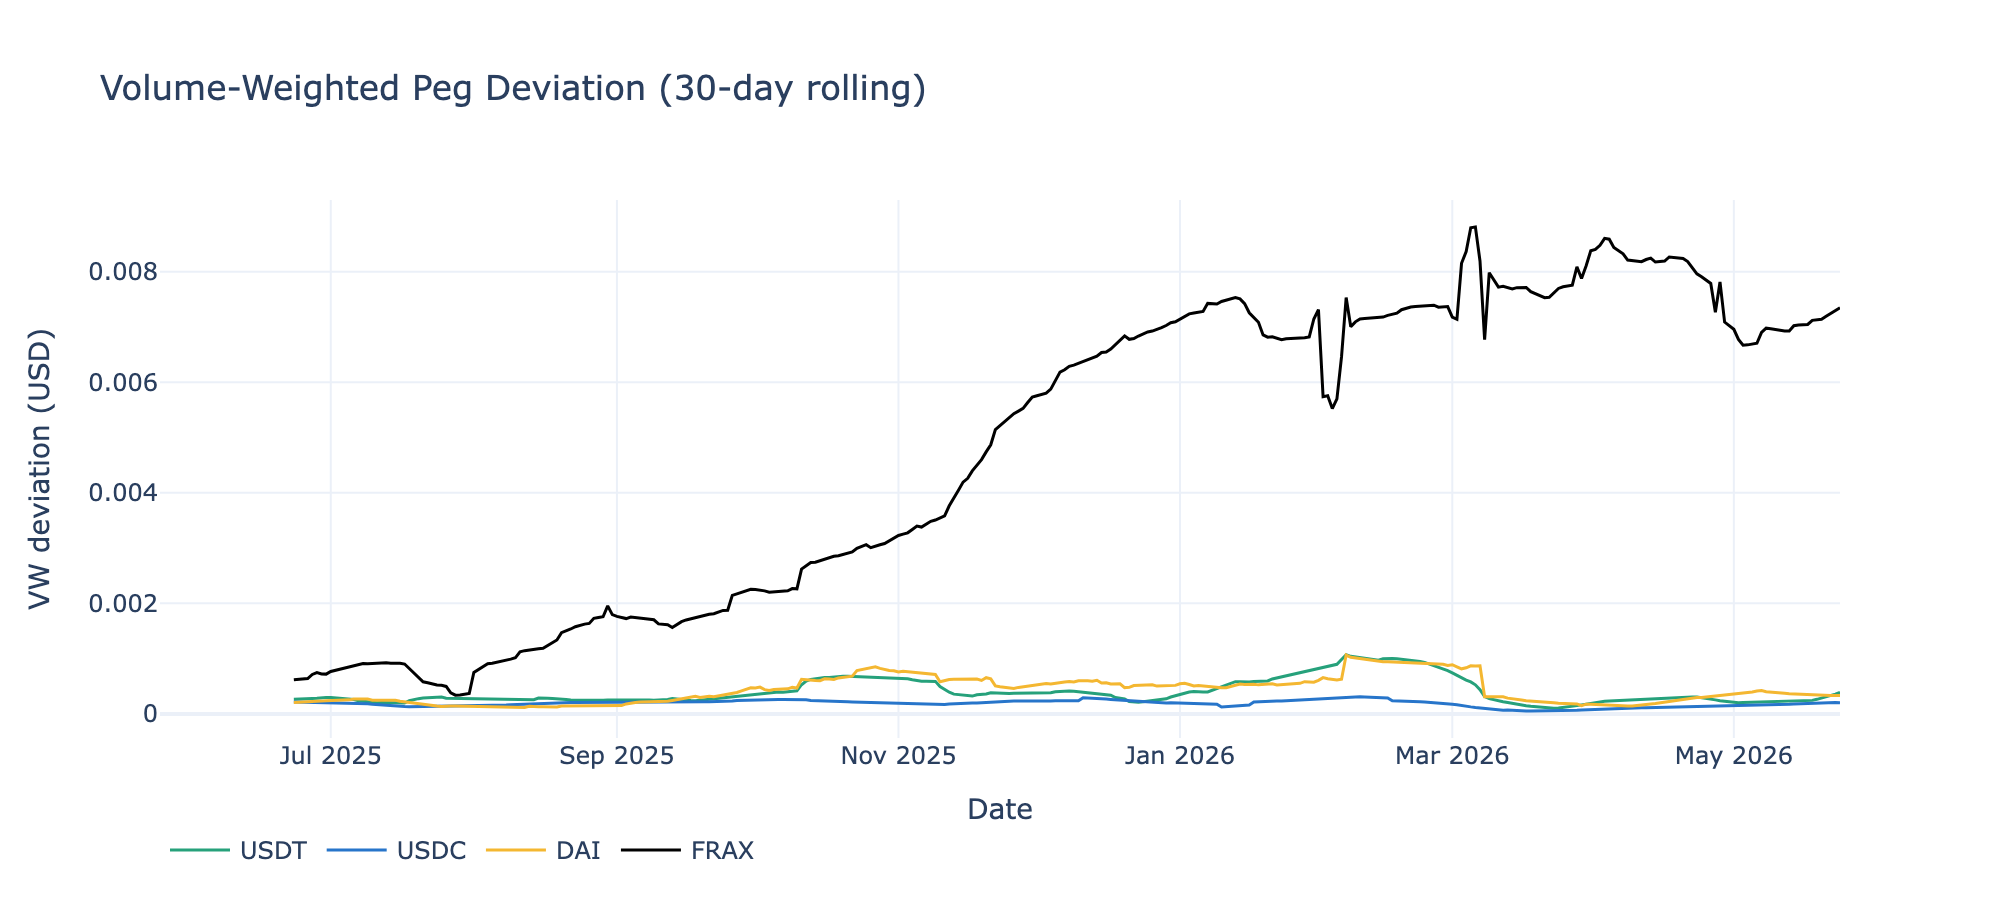
\includegraphics[width=\columnwidth]{vw_deviation.png}
\caption{Thirty-day volume-weighted peg deviation.}
\label{fig:vwdev}
\end{figure}

\section{Market Stress Correlation}
Broad crypto-market stress is proxied by the absolute daily BTC return. This follows prior evidence that stablecoin premiums, discounts, issuance, and arbitrage can interact with broader crypto-market liquidity and stress~\cite{lyons_2023_stablecoins,ante_2021_issuance}. Fig.~\ref{fig:btccorr} overlays normalized BTC price behavior with stablecoin peg deviations. The notebook also computes Pearson correlations between $|\Delta BTC|$ and each stablecoin's deviation. This diagnostic tests whether peg stress behaves as an isolated asset-specific event or clusters with broader market volatility.

\begin{figure}[t]
\centering
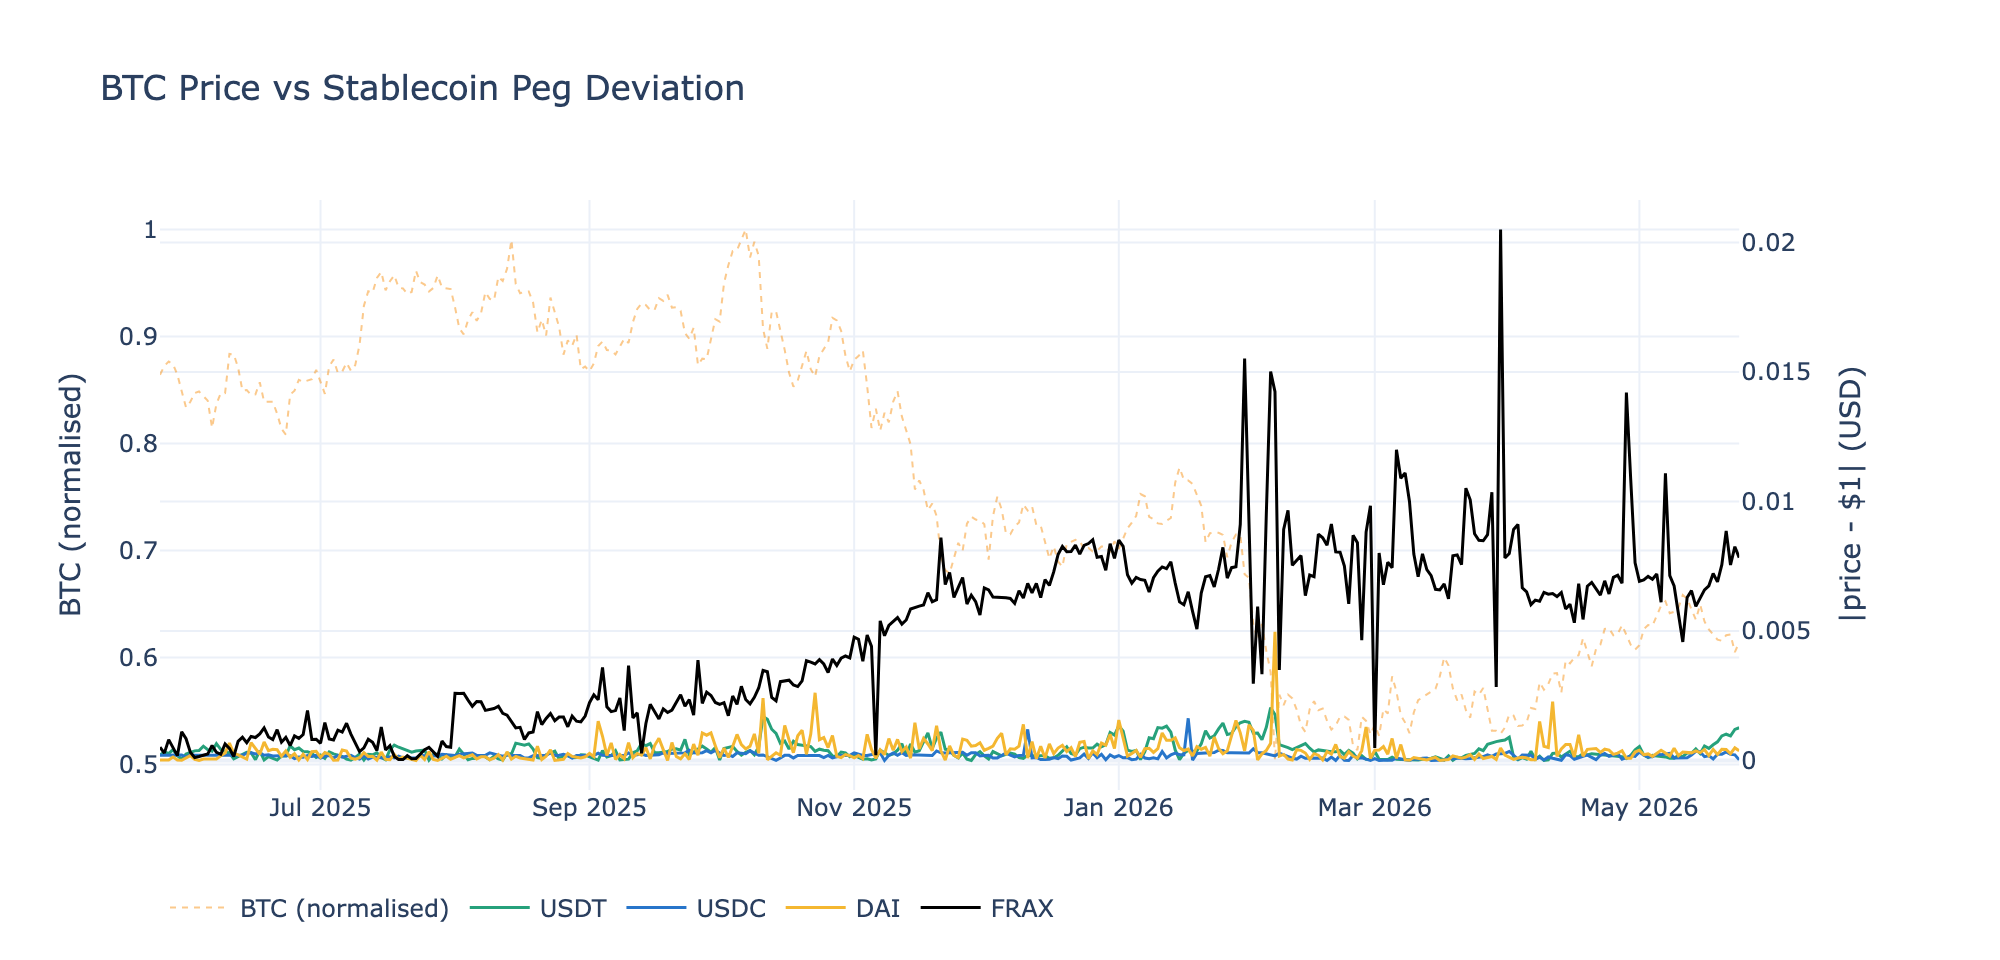
\includegraphics[width=\columnwidth]{btc_correlation.png}
\caption{BTC price behavior versus stablecoin peg deviation.}
\label{fig:btccorr}
\end{figure}

\section{Risk Interpretation}
The empirical findings motivate a mechanism-specific interpretation.

\subsection{Fiat-Collateralized Stablecoins}
USDT and USDC show the tightest routine peg behavior in the repository analysis. This supports their use as low-noise settlement assets under normal conditions. However, observed daily volatility does not fully capture their main risk: a discontinuous shock can arise from issuer, banking, custodian, reserve, regulatory, or redemption-channel failures~\cite{gorton_zhang_2023_wildcat,fsb_2023_gsc}. Historical episodes such as USDC's March 2023 Silicon Valley Bank-linked de-peg illustrate that fiat-backed designs can experience rapid but short-lived peg breaks when confidence in reserve accessibility is impaired~\cite{circle_svb_update}. This event is a contextual example; it is not necessarily inside a rolling 365-day sample unless the notebook is executed over a period that includes March 2023.

\subsection{Crypto-Collateralized Stablecoins}
DAI exhibits slightly wider baseline deviation in the documented results. The tradeoff is observability: collateral composition, vault parameters, liquidation conditions, and governance changes are more transparent than in a purely off-chain reserve model~\cite{makerdao_whitepaper,kozhan_2021_dai}. For a risk manager, observable risk can be easier to monitor and hedge than opaque reserve risk, even when day-to-day price variance is higher.

\subsection{Hybrid Stablecoins}
FRAX shows the widest deviation behavior in the repository findings. Hybrid or fractional designs can introduce reflexivity: if part of the stabilizing mechanism depends on crypto-native collateral or governance-token value, that support can weaken during market stress. Evidence from algorithmic and partially endogenous stablecoin runs shows how redemption pressure can become self-reinforcing when confidence in the stabilizing asset collapses~\cite{adams_ibert_2022_runs,klages_2020_stablecoins2}. This creates a risk profile that should not be grouped with fiat-backed stablecoins in a portfolio model~\cite{frax_docs}.

\section{Capital Allocation Implications}
The main allocation result is that stablecoin exposure should be disaggregated by mechanism. A DeFi yield book should not hold a single undifferentiated ``stablecoin'' bucket. Instead, risk limits should separate fiat-backed, crypto-collateralized, and hybrid designs, with each bucket monitored by deviation, liquidity, redemption, and recovery metrics. This is consistent with policy recommendations that focus on reserve quality, enforceable redemption claims, governance, operational resilience, and risk management for stablecoin arrangements~\cite{fsb_2023_gsc,pwg_2021_stablecoins}.

Second, peg deviation should be treated as a real-time risk signal. A rising rolling deviation or volume-weighted deviation can justify reducing exposure, widening collateral haircuts, rebalancing toward more liquid assets, or temporarily lowering leverage in protocols that rely on stablecoin collateral. This matters because DeFi protocols can transmit shocks through collateral reuse, liquidations, and automated leverage~\cite{schar_2021_defi,bis_2022_future_monetary,imf_2021_gfsr}.

Third, statistical separation matters. The reported Kruskal-Wallis significance at $p<0.05$ implies that the four deviation distributions should not be pooled without losing important risk information. This supports mechanism-specific capital charges or exposure caps rather than a uniform assumption that all assets priced near \$1 have identical risk.

\section{Limitations}
The analysis uses daily data and therefore may miss intraday de-pegs, fast recovery dynamics, and transient exchange-specific liquidity shocks. CoinGecko aggregates market data across venues, which is useful for broad measurement but may differ from executable prices in a particular DeFi pool or centralized exchange. The rolling 365-day sample also means that re-running the notebook changes the empirical window. For auditability, future versions should persist raw downloaded data, exact execution dates, and numeric result tables alongside the charts.

\section{Conclusion}
This paper presents an IEEE-style empirical report for a DeFi stablecoin peg-stability study. The results show that major stablecoins maintain the \$1 peg with different levels of tightness and different failure modes. Fiat-backed assets show low normal-day deviation but concentrated off-chain tail risk; DAI trades higher baseline noise for greater on-chain observability; and FRAX carries wider and more reflexive peg risk. These differences are visible in the deviation distributions, rolling volatility, volume-weighted deviation, and market-stress diagnostics. The practical implication is clear: risk-aware DeFi capital allocation should classify stablecoins by mechanism, monitor peg deviation dynamically, and avoid treating all dollar-pegged assets as interchangeable cash.

\section*{Reproducibility}
The analysis notebook is provided as \texttt{stablecoin\_peg\_analysis.ipynb}. Re-running the notebook fetches current CoinGecko data and refreshes the figures under \texttt{charts/}. The LaTeX source for this paper is stored under \texttt{paper/}.

\bibliographystyle{IEEEtran}
\bibliography{references}

\end{document}
